\section{Motivação}

\begin{frame}[fragile]{Máquinas idealizadas e máquinas reais}

    \begin{itemize}
        \item As máquinas de Turing e os ábacos são máquinas idealizadas

        \item Algumas de suas características não podem ser traduzidas diretamente
            para máquinas reais, como o fato da fita ser infinita em um máquina de Turing, ou
            de um registrador de um ábaco armazenar um inteiro de tamanho arbitrário

        \item Além disso, o conjunto de instruções para estas máquinas idealizadas é mínimo,
            de modo que escrever programas, mesmo simples, se torna uma tarefa árdua e demorada

        \item Em 1945, um novo passo foi dado em direção da construção de máquinas reais, pelo
            matemático e físico John Von Neumann
    \end{itemize}

\end{frame}

\begin{frame}[fragile]{Arquitetura de Von Neumann}

    \begin{itemize}
        \item A \textbf{arquitetura de Von Neumann} (ou arquitetura de Princeton), descreve a 
            arquitetura básica para um computador digital eletrônico

        \item Ela é composta por um unidade lógico-aritmética (\textit{arithmetic logic unit} -- 
            ALU) e registradores de processador,
            uma unidade de controle contendo um registrador de instrução e um contador de 
            programa (\textit{program counter} -- PC), uma unidade de memória para armazenar o 
            programa e as instruções, uma
            memória externa e mecanismos de entrada e saída de dados

        \item Esta arquitetura foi o alicerce que deu origem aos computadores modernos que, 
            embora mais elaborados e sofisticados, em grande parte ainda seguem esta arquitetura
            básica
    \end{itemize}

\end{frame}

\begin{frame}[fragile]{Visualização da arquitetura de Von Neumann}

    \renewcommand{\figurename}{Fonte}
    \begin{figure}[ht]
        \centering
        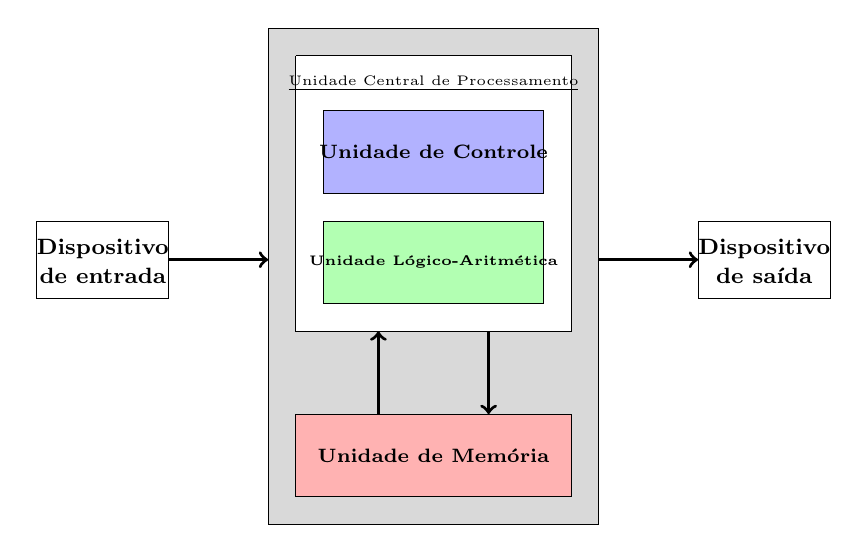
\begin{tikzpicture}[scale=0.7]
            \node at (-1, 4) { \footnotesize \textbf{Dispositivo} };
            \node at (-1, 3.5) { \footnotesize \textbf{de entrada} };

            \node at (11, 4) { \footnotesize \textbf{Dispositivo} };
            \node at (11, 3.5) { \footnotesize \textbf{de saída} };

            \coordinate (A1) at (-2.2, 4.5);
            \coordinate (B1) at (0.2, 4.5);
            \coordinate (C1) at (0.2, 3.1);
            \coordinate (D1) at (-2.2, 3.1);

            \draw (A1) -- (B1) -- (C1) -- (D1) -- (A1);

            \coordinate (A2) at (2, 8);
            \coordinate (B2) at (8, 8);
            \coordinate (C2) at (8, -1);
            \coordinate (D2) at (2, -1);

            \draw[fill=gray!30] (A2) -- (B2) -- (C2) -- (D2) -- (A2);

            \coordinate (A3) at (9.8, 4.5);
            \coordinate (B3) at (12.2, 4.5);
            \coordinate (C3) at (12.2, 3.1);
            \coordinate (D3) at (9.8, 3.1);

            \draw (A3) -- (B3) -- (C3) -- (D3) -- (A3);

            \draw[->,very thick] (0.2, 3.8) -- (2, 3.8);
            \draw[->,very thick] (8, 3.8) -- (9.8, 3.8);

            \coordinate (A4) at (2.5, 7.5);
            \coordinate (B4) at (7.5, 7.5);
            \coordinate (C4) at (7.5, 2.5);
            \coordinate (D4) at (2.5, 2.5);

            \draw[fill=white] (A4) -- (B4) -- (C4) -- (D4) -- (A4);
            \node at (5, 7) { \tiny \underline{Unidade Central de Processamento} };

            \coordinate (A5) at (3, 6.5);
            \coordinate (B5) at (7, 6.5);
            \coordinate (C5) at (7, 5);
            \coordinate (D5) at (3, 5);

            \draw[fill=blue!30!white] (A5) -- (B5) -- (C5) -- (D5) -- (A5);
            \node at (5, 5.75) { \scriptsize \bf {Unidade de Controle} };

            \coordinate (A6) at (3, 4.5);
            \coordinate (B6) at (7, 4.5);
            \coordinate (C6) at (7, 3);
            \coordinate (D6) at (3, 3);

            \draw[fill=green!30!white] (A6) -- (B6) -- (C6) -- (D6) -- (A6);
            \node at (5, 3.75) { \tiny \bf {Unidade Lógico-Aritmética} };

            \coordinate (A7) at (2.5, 1.0);
            \coordinate (B7) at (7.5, 1.0);
            \coordinate (C7) at (7.5, -0.5);
            \coordinate (D7) at (2.5, -0.5);

            \draw[fill=red!30!white] (A7) -- (B7) -- (C7) -- (D7) -- (A7);
            \node at (5, 0.25) { \scriptsize \bf {Unidade de Memória} };

            \draw[->,very thick] (4, 1) -- (4, 2.5);
            \draw[<-,very thick] (6, 1) -- (6, 2.5);
        \end{tikzpicture}

        \caption{\href{https://upload.wikimedia.org/wikipedia/commons/e/e5/Von_Neumann_Architecture.svg}{Wikipédia}, com adaptações.}
    \end{figure}
\end{frame}

\begin{frame}[fragile]{Linguagem de Máquina}

    \begin{itemize}
        \item As máquinas reais dispõem de dispositivos internos (sejam mecânicos, elétricos ou
            eletrônicos) que permitem a realização de tarefas básicas (somas, operações lógicas,
            etc)

        \item Nas primeiras máquinas reais, para montar um programa que resolvesse um problema 
            específico era preciso reconfigurar fisicamente tais equipamentos

        \item A medida que estas máquinas foram evoluindo, códigos binários foram associadas à 
            estas tarefas (instruções) básicas, de modo que era possível escrever novos programas
            sem modificar o hardware fisicamente, inserindo tais sequências de zeros e uns por
            meio de \textit{switches}

        \item Estas códigos binários constituem a \textbf{linguagem de máquina} do hardware

        \item Mesmo com todo este avanço, escrever programas não eram muito mais fácil ou simples
            do que escrever programas para ábacos ou máquinas de Turing
    \end{itemize}

\end{frame}

\begin{frame}[fragile]{Linguagem Assembly}

    \begin{itemize}
        \item Logo os programadores entenderam que era mais fácil associar os códigos binários
            das instruções a mnemônicos

        \item Estes mnemônicos representavam tanto as instruções em si quanto as principais 
            localizações de memória

        \item Assim foram desenvolvidas, a partir dos anos 1950, as linguagens Assembly

        \item Para cada linguagem era criado um \textit{assembler} (montador), que consistia em 
            uma ferramenta de software que traduzia estes mnemônicos em linguagem de máquina

        \item Cada arquitetura e cada hardware em particular oferecia um conjunto distinto de
            instruções, de modo que para cada um deles era necessária uma linguagem Assembly
            distinta

        \item Embora elas representem um avanço considerável em relação aos ábacos, as linguagens
            Assembly carecem da abstração presente na notação matemática convencional
    \end{itemize}

\end{frame}
